\documentclass{beamer}
\usepackage{ragged2e}
\usepackage{graphicx}
% Theme
\usetheme[block=fill, progressbar=frametitle]{metropolis} % Choose a theme (e.g., "Madrid", "Warsaw", "CambridgeUS", "Boadilla", etc.)
\usecolortheme{spruce}

\setbeamercolor{background canvas}{bg=white}
% Title
\title{Rectangular Partitioning of Rectilinear Polygons}
\subtitle{Exercise 15}
\author{Alexandre Ros}
\date{\today}
% Begin the document
\begin{document}

% Title page
\frame{\titlepage}

% Table of Contents
% \begin{frame}
%    \frametitle{Table of Contents}
%    \tableofcontents
%\end{frame}

% Section 1
\section{Introduction to the problem}

\begin{frame}{Introduction}
	\begin{block}{Exercise 15}
	\textbf{Decompose a rectilinear polygon into rectangles}, using segments aligned with the edges of the polygon.
The algorithm must produce the \textbf{minimum number of pieces}, and the output must give a
complete description of the partition.
	\end{block}
	\begin{block}{Input}
	A polygon whose sides meet at right angles.
	\end{block}  
	\begin{block}{Output}
	A \textbf{partition} of the polygon into rectangles, with no overlaps.
	\end{block}
\end{frame}

\begin{frame}{Examples}
\begin{figure}
\centering
  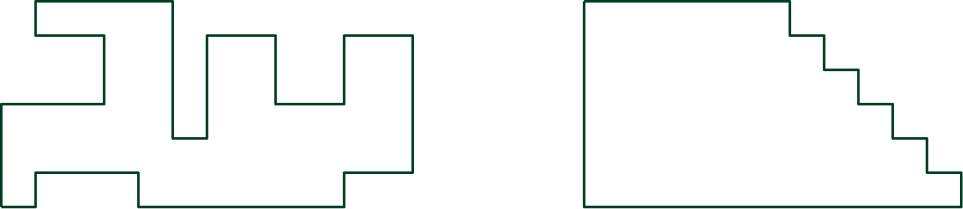
\includegraphics[width=.8\textwidth]{"./rect1.png"}
  \caption{Two rectilinear polygons.}
     \label{fig:question}
\end{figure}
\begin{figure}
\centering
  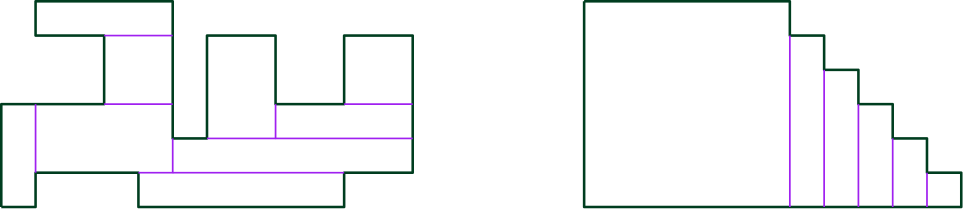
\includegraphics[width=.8\textwidth]{"./rec1sol.png"}
  \caption{A minimum partition of both.}
     \label{fig:question}
\end{figure}

\end{frame}


% Section 2
\section{Solution}

\begin{frame}[t]{Main Content}
    \begin{block}{Important Point}
        This is an important point you want to highlight.
    \end{block}
    \begin{itemize}
        \item More content.
        \item More points.
    \end{itemize}
\end{frame}

% Section 3
\section{Conclusion}

\begin{frame}
    \frametitle{Conclusion}
    \begin{itemize}
        \item Summarize key points.
        \item Highlight takeaways.
    \end{itemize}
\end{frame}

% Additional slides, if needed

% Thank you slide
\begin{frame}
    \frametitle{Thank You}
    \centering
    \Huge Thank you for your attention!
\end{frame}

\end{document}
